\graphicspath{ {images/} }

\titledquestion{Attention Exploration}[14]
\label{sec:analysis}

Multi-head self-attention is the core modeling component of Transformers.
In this question, we'll get some practice working with the self-attention equations, and motivate why multi-headed self-attention can be preferable to single-headed self-attention.

Recall that attention can be viewed as an operation on a \textit{query} vector $q\in\mathbb{R}^d$, a set of \textit{value} vectors $\{v_1,\dots,v_n\}, v_i\in\mathbb{R}^d$, and a set of \textit{key} vectors $\{k_1,\dots,k_n\}, k_i \in \mathbb{R}^d$, specified as follows:
\begin{align}
&c = \sum_{i=1}^{n} v_i \alpha_i \\
&\alpha_i = \frac{\exp(k_i^\top q)}{\sum_{j=1}^{n} \exp(k_j^\top q)}
\end{align} 
with $alpha = \{\alpha_1, \ldots, \alpha_n\}$ termed the ``attention weights''. 
Observe that the output $c\in\mathbb{R}^d$ is an average over the value vectors weighted with respect to $\alpha$.

\begin{parts}

\part[3] \label{copying} \textbf{Copying in attention.} One advantage of attention is that it's particularly easy to ``copy'' a value vector to the output $c$. In this problem, we'll motivate why this is the case.

\begin{subparts}
    \subpart[2] The distribution $\alpha$ is typically relatively ``diffuse''; the probability mass is spread out between many different $\alpha_i$. However, this is not always the case. \textbf{Describe} (in one sentence) under what conditions the categorical distribution $\alpha$ puts almost all of its weight on some $\alpha_j$, where $j \in \{1, \ldots, n\}$ (i.e. $\alpha_j \gg \sum_{i \neq j} \alpha_i$). What must be true about the query $q$ and/or the keys $\{k_1,\dots,k_n\}$?

    \ifans{For a single attention weight to dominate, the dot product between the query vector $q$ and the key $k_j$, $k_j^{\top}q$, has to be much larger than all other $k_i^{\top}q$ for $i\ne i$. }

    \subpart[1] Under the conditions you gave in (i), \textbf{describe} the output $c$. 

    \ifans{Under that condition, the output $c$ is essentially the value vector $v_j$ as $\alpha_j \gg \alpha_{i \ne j}$. }

\end{subparts}


\part[2]\textbf{An average of two.} 
\label{q_avg_of_two}
Instead of focusing on just one vector $v_j$, a Transformer model might want to incorporate information from \textit{multiple} source vectors.

Consider the case where we instead want to incorporate information from \textbf{two} vectors $v_a$ and $v_b$, with corresponding key vectors $k_a$ and $k_b$.
Assume that (1) all key vectors are orthogonal, so $k_i^\top k_j = 0$ for all $i \neq j$; and (2) all key vectors have norm $1$.
\textbf{Find an expression} for a query vector $q$ such that $c \approx \frac{1}{2}(v_a + v_b)$, and \textbf{justify your answer}.\footnote{Hint: while the softmax function will never \textit{exactly} average the two vectors, you can get close by using a large scalar multiple in the expression.} (Recall what you learned in part~(\ref{copying}).)

\ifans{From the expression of the output vector $c$, we see that $\alpha_a=\alpha_b=1/2$. This means $k_a^{\top}q=k_b^{\top}q$. Given $k_i^{\top}k_j=0$, if we have $q=\lambda(k_a+k_b)$ for some constant $\lambda$, we have $k_a^{\top}q=k_b^{\top}q$.

For other key vectors $k_i$ where $i \notin \{a,b\}$, we have $k_i^{\top}q=0$. Therefore, 
\begin{equation*}
    \alpha_a=\alpha_b=\frac{e^{\lambda}}{2e^{\lambda}+\sum_{i \ne a,b}e^0} = \frac{e^\lambda}{2e^\lambda+(n-2)}.
\end{equation*}
As $\lambda$ becomes large, we have $\alpha_a=\alpha_b \approx \frac{1}{2}$. Therefore, $q=\lambda(k_a+k_b)$ for some large $\lambda$.
}

\part[5]\textbf{Drawbacks of single-headed attention:} \label{q_problem_with_single_head}
In the previous part, we saw how it was \textit{possible} for a single-headed attention to focus equally on two values.
The same concept could easily be extended to any subset of values.
In this question we'll see why it's not a \textit{practical} solution.

Consider a set of key vectors $\{k_1,\dots,k_n\}$ that are now randomly sampled, $k_i\sim \mathcal{N}(\mu_i, \Sigma_i)$, where the means $\mu_i \in \mathbb{R}^d$ are known to you, but the covariances $\Sigma_i$ are unknown (unless specified otherwise in the question).
Further, assume that the means $\mu_i$ are all perpendicular; $\mu_i^\top \mu_j = 0$ if $i\not=j$, and unit norm, $\|\mu_i\|=1$.

\begin{subparts}
\subpart[2] Assume that the covariance matrices are $\Sigma_i = \alpha I, \forall i \in \{1, 2, \ldots, n\}$, for vanishingly small $\alpha$.
Design a query $q$ in terms of the $\mu_i$ such that as before, $c\approx \frac{1}{2}(v_a + v_b)$, and provide a brief argument as to why it works.

\ifans{We can write the key vector $k_i$ drawn from normal distribution as $k_i=\mu_i+\epsilon_i$, where $\epsilon_i \sim \mathcal{N}(0,\Sigma_i)$. To get $\alpha_a\approx\alpha_b\approx \frac{1}{2}$, we need $k_a^{\top}q\approx k_b^{\top}q$ and $k_{i\ne a,b}^{\top}q \approx0$.

Try $q=\lambda(\mu_a+\mu_b)$, we have 
\begin{equation*}
    \mathbb{E}[k_i^{\top}q]=\mathbb{E}[k_i]^{\top}q= \mu_i^\top q = \begin{cases}
        \lambda & i \in \{a,b\}\\
        0 & i \notin \{a,b\} 
    \end{cases}
\end{equation*}
and 
\begin{align*}
    \text{Var}(q^{\top}k_i) &= \text{Var}(q^\top \mu_i+q^\top \epsilon_i)=\text{Var}(q^\top \epsilon_i) \\
    &= \mathbb{E}[(q^\top \epsilon_i- \mathbb{E}[q^\top \epsilon_i])^2] = \mathbb{E}[(q^\top \epsilon_i)^2] = \mathbb{E}[q^\top \epsilon_i\epsilon_i^{\top}q] \\
    &= q^\top \mathbb{E}[\epsilon_i\epsilon_i^\top]q = q^\top(\alpha I)q = \alpha q^\top q = \alpha(2\lambda^2)
\end{align*}
Therefore, for vanishingly small $\alpha$, we have the variance term tending to zero, giving $\alpha_a \approx \alpha_b \approx \frac{1}{2}$. In other words, the only randomness is small, isotropic noise, making the key vectors hover stably around the mean. 
}

\subpart[3] Though single-headed attention is resistant to small perturbations in the keys, some types of larger perturbations may pose a bigger issue. In some cases, one key vector $k_a$ may be larger or smaller in norm than the others, while still pointing in the same direction as $\mu_a$.\footnote{Unlike the original Transformer, newer Transformer models apply layer normalization before attention. In these pre-layernorm models, norms of keys cannot be too different which makes the situation in this question less likely to occur.}

As an example, let us consider a covariance for item $a$ as $\Sigma_a = \alpha I + \frac{1}{2}(\mu_a\mu_a^\top)$ for vanishingly small $\alpha$ (as shown in figure \ref{ka_plausible}). This causes $k_a$ to point in roughly the same direction as $\mu_a$, but with large variances in magnitude. Further, let $\Sigma_i = \alpha I$ for all $i \neq a$.
\begin{figure}[h]
\centering
\captionsetup{justification=centering,margin=2cm}
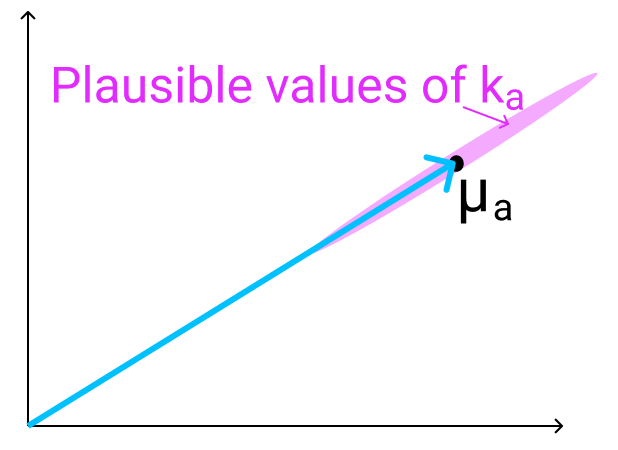
\includegraphics[width=0.35\linewidth]{images/ka_plausible.png}
\caption{The vector $\mu_a$ (shown here in 2D as an example), with the range of possible values of $k_a$ shown in red. As mentioned previously, $k_a$ points in roughly the same direction as $\mu_a$, but may have larger or smaller magnitude.}
\label{ka_plausible}
\end{figure}

When you sample $\{k_1,\dots,k_n\}$ multiple times, and use the $q$ vector that you defined in part i., what do you expect the vector $c$ will look like qualitatively for different samples? Think about how it differs from part (i) and how $c$'s variance would be affected.

\ifans{The difference of this situation is the covariance matrix $\Sigma_a$, which means the magnitude of the key vector $k_a$ can fluctuate a lot. Since the magnitude of $k_a$ affects $q^\top k_a$, the attention score $\alpha_a$ will be large if $k_a$ has a large magnitude, vice versa. This introduces a large variance in the output $c$, which fluctuates and is no longer stable.

Mathematically, we have 
\begin{align*}
    \text{Var}(q^\top k_a) &= \text{Var}(q^\top \epsilon_a) = q^\top (\alpha I +\frac{1}{2}\mu_a \mu_a^\top)q \\
    &= 2a\lambda^2 + \frac{1}{2}\lambda^2 = (2\alpha+\frac{1}{2})\lambda^2. \\
    \text{Var}(q^\top k_i) &= 2a\lambda^2, i \ne a
\end{align*}
This proves that the variance of $q^\top k_a$ is no longer vanishingly small, thus the variance of $\alpha_a$ is not negligible. The output vector $c$ does is not stably $\frac{1}{2}(v_a+v_b)$.
}
\end{subparts}

\part[3]\textbf{Benefits of multi-headed attention:} \label{q_multi_head}
Now we'll see some of the power of multi-headed attention.
We'll consider a simple version of multi-headed attention which is identical to single-headed self-attention as we've presented it, except two query vectors ($q_1$ and $q_2$) are defined, which leads to a pair of vectors ($c_1$ and $c_2$), each the output of single-headed attention given its respective query vector.
The final output of the multi-headed attention is their average, $\frac{1}{2}(c_1+c_2)$.

As in question 1(\ref{q_problem_with_single_head}), consider a set of key vectors $\{k_1,\dots,k_n\}$ that are randomly sampled, $k_i\sim \mathcal{N}(\mu_i, \Sigma_i)$, where the means $\mu_i$ are known to you, but the covariances $\Sigma_i$ are unknown.
Also as before, assume that the means $\mu_i$ are mutually orthogonal; $\mu_i^\top \mu_j = 0$ if $i\not=j$, and unit norm, $\|\mu_i\|=1$.

\begin{subparts}
\subpart[1]
Assume that the covariance matrices are $\Sigma_i=\alpha I$, for vanishingly small $\alpha$.
Design $q_1$ and $q_2$ in terms of $\mu_i$ such that $c$ is approximately equal to $\frac{1}{2}(v_a+v_b)$. 
Note that $q_1$ and $q_2$ should have different expressions.

\ifans{$c=\frac{1}{2}(c_1+c_2)$. Therefore, we can have $c_1=v_a$ and $c_2=v_b$. This requires $q_1=\lambda_1(k_a)$ and $q_2=\lambda_2(k_b)$.
}

\subpart[2]
Assume that the covariance matrices are $\Sigma_a=\alpha I + \frac{1}{2}(\mu_a\mu_a^\top)$ for vanishingly small $\alpha$, and $\Sigma_i=\alpha I$  for all $i \neq a$.
Take the query vectors $q_1$ and $q_2$ that you designed in part i.
What, qualitatively, do you expect the output $c$ to look like across different samples of the key vectors? Explain briefly in terms of variance in $c_1$ and $c_2$. You can ignore cases in which $k_a^\top q_i < 0$.

\ifans{
From the above investigations, we can conclude that for head 1, we have 
\begin{align*}
    \text{Var}(q_1^\top k_a) &= (2\alpha+1/2)\lambda_1^2 \\
    \text{Var}(q_1^\top k_i) &= 2\alpha \lambda^2, i \ne a
\end{align*}.
For head 2, we have $\text{Var}(q_1^\top k_i) = 2\alpha \lambda^2$ for all $i$. Therefore, $c_2$ has vanishingly small variance, while $c_1$ has a non-negligible variance. The variance of $c=\frac{1}{2}(c_1+c_2)$, which is the average of $c_1$ and $c_2$, has lower variance compared to the noisy head, head 1.
}
\end{subparts}

\part[1] Based on part~(\ref{q_multi_head}), briefly summarize how multi-headed attention overcomes the drawbacks of single-headed attention that you identified in part~(\ref{q_problem_with_single_head}).

\ifans{In conclusion, multi-head attention allows different heads to focus on different subspaces/items, e.g. $a$ and $b$, without needing a single finely tuned query. Then, averaging heads stabilizes the output and reduces the variances of individual key vectors that are noisy in norm. Therefore, multi-head represents a mixture of values, which is more robust to key perturbations than a single head.}

\end{parts}
